\documentclass[notes]{beamer} % notes=only for notes, frames
\usetheme{metropolis}

\usepackage{amsmath,amsfonts}
\usepackage{graphicx}
\usepackage{hyperref}
\usepackage{tikz}
\usetikzlibrary {positioning}
\usetikzlibrary{arrows.meta}
\usetikzlibrary {automata}

\input{sym}

\title[DRL for DL experts]{Deep Reinforcement Learning for deep learning experts}
\author{Vikas Dhiman}

\begin{document}
\maketitle

\begin{frame}
  Prerequisites for knowing Reinforcement Learning
  \begin{enumerate}
    \item Linear algebra 
    \item Probability
    \item Python
  \end{enumerate}

  Prerequisites for knowing Deep Reinforcement Learning
  \begin{enumerate}
  \item Deep Learning
  \end{enumerate}
\end{frame}

\begin{frame}{BF Skinner's Reinforcement Learning for Pigeons}
  \centering
  \href{http://bfskinner.org/wp-content/uploads/2015/02/Operant_Conditioning.mp4}{Video}\\
  \includegraphics[width=0.45\linewidth]{media/pigeon-peck.png}%
  \includegraphics[width=0.45\linewidth]{media/pigeon-turn.png}
  \footnote{Image source:bfskinner.org}

\end{frame}

\note{
  \begin{enumerate}
  \item BF Skinner demonstrated that pigeons could learn to repeat an action
    that lead them to a particular reward.
    \cite[p15]{sutton2020reinforcement}
  \end{enumerate}
}

\begin{frame}{RL terminology}
  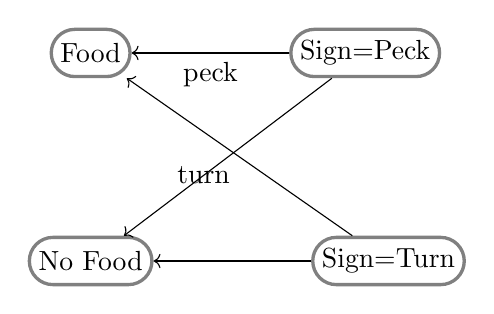
\begin{tikzpicture}[node distance=20mm,
    state/.style={
      % The shape:
      rectangle,minimum size=6mm,rounded corners=3mm,
      % Border
      very thick,draw=black!50
      }]
  \node (food) [state] {Food};
  \node (no-food) [state, below=of food] {No Food};
  \node (sign-peck) [state,right=of food] {Sign=Peck};
  \node (sign-turn) [state,right=of no-food] {Sign=Turn};
  \draw [->] (sign-peck) to [edge label=peck] (food);
  \draw [->] (sign-peck) to (no-food);
  \draw [->] (sign-turn) to [edge label=turn] (food);
  \draw [->] (sign-turn) to (no-food);
  \end{tikzpicture}
  \begin{description}
  \item[State ] ($\bfs_t \in \calS$) Example: Sign is peck or turn. Food is
    dispensed or not.
  \item[Reward function ] ($r_t(\bfs_t) \to \bbR$) Example: Food is high reward ($r_t = 100$).
food is zero-reward ($r_t = 0$).
\item[Actions ] ($\bfa_t \in \calA$) Example: To peck or to turn or no action.
  \item[Transition probabilities]
    ($T(\bfs_{t+1}|\bfs_{t}, \bfa_t) \to [0, 1 ] $) Example:
    Probability of food dispensing if you peck when Sign-peck is shown.
  \end{description}
\end{frame}
\note{
  State is the full description of the world at time $t$ that captures the
entire history. Example: in this example the state can be captured with two bits
$\bfs_t = [f_t; p_t]$, where $f_t \in \{0, 1\}$ describes a food or no food
state and $p_t \in \{0, 1\}$ describes the sign showing  peck or turn.
}

\begin{frame}{Better state diagram}
  \begin{tikzpicture}[node distance=20mm,
    state/.style={
      % The shape:
      rectangle,minimum size=6mm,rounded corners=3mm,
      % Border
      very thick,draw=black!50
    },
    every to/.style={
      thick,bend right
    }
    ]
    \node (food-turn) [state] {Food/Sign=Turn};
    \node (food-peck) [state, below=of food] {Food/Sign=Peck};
    \node (no-food-turn) [state,right=of food] {NoFood/Sign=Turn};
    \node (no-food-peck) [state,right=of no-food] {NoFood/Sign=Peck};
    \draw [-Stealth](no-food-turn) to [edge label=turn] (food-turn);
    \draw [-Stealth](no-food-peck) to [edge label=peck] (food-peck);
    \draw [-Stealth](food-turn) to [edge label=eat] (no-food-turn);
    \draw [-Stealth](food-peck) to [edge label=eat] (no-food-peck);
    \draw [-Stealth](no-food-turn) to [edge label=?] (no-food-peck);
    \draw [-Stealth](no-food-peck) to [edge label=?] (no-food-turn);
    \draw [-Stealth] (no-food-turn.north) to [in=45,out=-45,loop,edge label'=peck] (no-food-turn.north);

    \draw [-Stealth] (no-food-peck.south) to [in=135,out=-135,loop,edge label=turn] (no-food-peck.south);
  \end{tikzpicture}
  
\end{frame}

\begin{frame}{RL problem}
  \begin{description}
      \item[Policy function] 
        $\pi(\bfs_t) \to \bfa_t$\\
      \item[Discount factor ] $\gamma \in (0,1)$.
  \end{description}
  \begin{align*}
    \pi^*(.) = \arg~\max_{\pi} \bbE_{T}\left[\sum_{t=0}^{\infty}
      \gamma^{t} r(\bfs_t) \right]
    \\
    \text{such that } \bfs_{t+1}\sim T(.|\bfs_t, \pi(\bfs_t))\forall t \in [k, \infty) \\
    \text{ and } \bfs_0 \sim p_0(.) 
  \end{align*}
\end{frame}

\begin{frame}{Value Function}
  \begin{align*}
    \pi^*(.) &= \arg~\max_{\pi} \bbE_{T}\left[\sum_{t=0}^{\infty}
    \gamma^{t} r(\bfs_t) \right]
    \\
    \text{such that }& \bfs_{t+1}\sim T(.|\bfs_t, \pi(\bfs_t)) \forall t \in [k, \infty)\\
    \text{ and }& \bfs_0 \sim p_0(.) 
  \end{align*}

  \begin{align*}
    V_\pi(\bfs_k) &= \bbE_{T}\left[\sum_{t=k}^{\infty}
    \gamma^{t} r(\bfs_t) \right]
    \\
    \text{such that }& \bfs_{t+1}\sim T(.|\bfs_t, \pi(\bfs_t)) \forall t \in [k, \infty)\\
  \end{align*}
\end{frame}

\begin{frame}{Action Value Function}
  \begin{align*}
    Q_\pi(\bfs_k, \bfa_k) &= \bbE_{T}\left[\sum_{t=k+1}^{\infty}
                    \gamma^{t} r(\bfs_t) \right]
    \\
    \text{such that }& \bfs_{t+1}\sim T(.|\bfs_t, \pi(\bfs_t)) \forall t \in [k, \infty) \\
  \end{align*}
\end{frame}


\begin{frame}{References}
\bibliography{main}
\bibliographystyle{abbrev}
\end{frame}
\end{document}
